\section{Étude de faisabilité}

\subsection{Carte embarquée}

\subsection{Énergie}

\subsubsection{Exigences}
\begin{itemize}

\item Autonomie: Les stations sont souvent situées dans des endroits très isolés et difficiles d'accès. Une solution est d'utiliser les ressources naturelles comme contribution à l'autonomie énergétique des stations et il est évident que la consommation électrique doit être minimale.

\smallskip \item Robustesse et Fiabilité: même en cas de problème environnemental l'approvisionnement de l'énergie à la station doit être assuré sans intervention humaine.

\smallskip \item Protection de l' environnement: les stations peuvent se trouver dans des espaces prot\'{e}g\'{e}s donc il faut mettre en place de l'\'{e}nergie non polluante et renouvelable car elle utilise des flux d'\'{e}nergie naturelle(soleil, vent, eau,croissance v\'{e}g\'{e}tale,...).
\end{itemize}

\subsubsection{Alternatives}
\begin{enumerate}
\item Énergie solaire photovolta\"ique
\begin{description}
\item [Avantages : ]
Les syst\`emes solaires photovoltaïques sont simples et rapides à installer, l'investissement  et le rendement sont pr\'{e}visibles à long terme.
Elle r\'{e}pond aux exigences de robustesse et de fiabilit\'{e} grâce à sa tolérance aux pannes et elle n\'{e}cessite tr\`es peu de maintenance. 
Elle est exploitable pratiquement partout, la lumi\`ere du soleil \'{e}tant disponible dans le monde entier. %Dans certains pays il fait nuit 6 mois l'année :p  
Aussi, cette production d'\'{e}nergie ne provoque aucune perturbation pour l' environnement.

\item [Risques et inconv\'enients : ]
Ces installations n\'{e}cessitant un apport en soleil, les pays proches des pôles, moins expos\'{e}s aux rayons solaires, sont tr\`es peu rentables.
\end{description}

\item Énergie \'{e}olienne
\begin{description}
\item [Avantages : ]
L'\'{e}nergie \'{e}olienne est renouvelable et est id\'{e}ale car il s'agit d une forme d'\'{e}nergie ind\'{e}finiment durable.
Elle ne produit pas de d\'{e}chets toxiques ou radioactifs. 
Son temps de fonctionnement est d'environ 20 ans.

\item [Risques et inconv\'{e}nients : ]
L'\'{e}nergie \'{e}olienne varie dans le temps.  Elle tourne uniquement s'il y a du vent.
La localisation des \'{e}oliennes est d\'{e}pendante de la ressource (le vent) et on ne peut pas les implanter n'importe où. 
Impact sur la faune, les \'{e}tudes ont constat\'{e} que des \'{e}oliennes \'{e}taient responsable de la mort de quelques oiseaux.
\end{description}


\item Batterie d' accumulateurs
\begin{description}
\item [Avantages : ]
Pour une alimentation sans interruption, les batteries stockent l'énergie permettant d'alimenter de quelques minutes à quelques heures.
Il existe les batteries rechargeables qui sont orient\'{e}es pour un fonctionnement avec des panneaux photovoltaïques ou  \'{e}oliennes(dur\'{e}e de vie augment\'{e}, propriét\'{e} anticorrosion grâces à des plaques positives \'{e}paisses, recyclable)

\item [Inconv\'{e}nients : ]
Le poids est important donc les frais de port peuvent s'av\'{e}rer cons\'{e}quents.
Polluant.

\end{description}
\end{enumerate}

\subsubsection{Choix de solution}
Après un analyse des exigences du syst\`eme nous proposons la combinaison de l'utilisation de batteries pour le stockage et pour la production une \'{e}nergie renouvelable pour satisfaire l'autonomie \'{e}nerg\'{e}tique.

\subsection{Capteurs}

    \subsubsection{Exigences}
    Les capteurs dont nous auront besoin doivent satisfaire à plusieurs
    contraintes principales: celle de la basse consommation d'énergie
    (et donc d'autonomie), celle de la précision, de la modularité (
    facilité de changement, de remplacement, de déplacement).

    \subsubsection{Solutions}
    La société française IJINUS conçoit ainsi des capteurs qui nous
    conviendraient: communicants, ils peuvent faire partie d'un
    réseau de capteurs. Ils sont en outre précis, et pas seulement
    pour des liquides en utilisant une mesure par imagerie acoustique.
    Ils sont de plus utilisables en environnement difficile, voire agressif.
    La tête de lecture est autonettoyante, permettant de ne pas avoir
    à intervenir si la tête est salle.

    \begin{figure}[!h]
    \begin{center}

    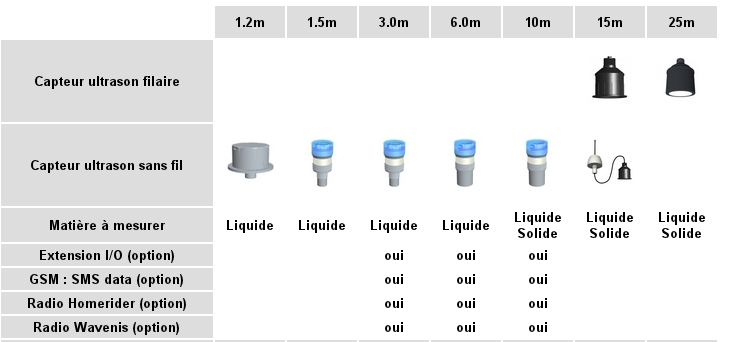
\includegraphics[width=15cm]{\PIXPATH/ijinus}
    \caption{Capteurs proposés par IJINUS}
    \end{center}
    \end{figure}

    Ce n'est pas la seule entreprise à proposer ce genre de matériel (comme la société SICK avec sa série LFVXXX), nous
    n'aurons donc a priori pas trop de mal à trouver notre bonheur au meilleur
    prix.

    \subsubsection{Conclusion}
    Le choix des capteurs demanderait une étude plus poussée
    pour trouver des capteurs correspondant précisément à nos besoins,
    ces capteurs pouvant être différents selon leur localisation.
    Les prix sont à discuter avec les fournisseurs.

\subsection{Communication}

Nous avons le choix entre plusieurs technologies différentes: la radiodiffusion, GSM, 3G, WiFi, etc.

\subsubsection{Transmetteurs radio – la radiodiffusion}

La radiodiffusion a la particularité de permettre une communication asymétrique. 
Une station de radio est une installation qui émet des ondes électromagnétiques à l'aide d'un émetteur radio et d'une antenne. 
Un poste de radio ou récepteur radio est un appareil permettant de recevoir les ondes radio, en extraire la modulation et restituer les sons sur un haut-parleur. 

Exemple d'émetteur adapté à notre but sur le marché: 

SOFREL BOX

\begin{figure}
\begin{center}

% sofrelbox.png

\end{center}
\end{figure}

Les transmetteurs SOFREL BOX sont spécifiquement développés pour le télé-contrôle de petites installations isolées et sans énergie.
Très simples à installer et à utiliser, les SOFREL BOX constituent une solution particulièrement adaptée pour les asservissements entre un site isolé et le serveur.
Ils permettent notamment :
\begin{description}
\item L’acquisition d’informations de contrôle (niveaux, compteurs,.…)
\item La communication inter-sites vers un poste local de télégestion SOFREL S500.
\end{description}
Doté d’un modem radio intégré le transmetteur déclenche un appel spontané vers le S500 de la station à chaque modification.
Hors alarme, les transmissions d’informations se font régulièrement selon une période paramétrable (toutes les 3, 5, 10 ou 15 minutes).

\subsubsection{Transmetteur GSM}

Exemple: CELLBOX

Développé pour la surveillance technique des sites dépourvus de source d’énergie et de toute liaison de communication filaire (RTC, LS/LP…), CELLBOX est un poste local de télégestion autonome communiquant par GSM (900/1800 Mhz).
CELLBOX assure l’acquisition et l’enregistrement d’informations d’alarmes, de comptages et de mesures, et effectue automatiquement différents calculs et bilans.
Étanche, CELLBOX intègre dans son boîtier une pile qui lui procure une autonomie totale de fonctionnement de plusieurs années.
Économique, simple et rapide à mettre en œuvre, CELLBOX apporte une solution performante pour répondre à de multiples applications : sectorisation de réseaux d’eau, recherche de fuites, télégestion de sites isolés...


\subsubsection{Transmetteur 3G/3G+}

Peu adapté, car le site doit avoir un réseau 3G.

Exemple : VIGICOM VID-1500

\begin{figure}
\begin{center}

% vigicom.png

\end{center}
\end{figure}

VigiCom VID-1500 est un transmetteur 3G spécialement étudié pour équiper tout véhicule ou site isolé. C’est un équipement complet de vidéo-surveillance temps réel par transmission via le réseau cellulaire (3G) réalisant une compression vidéo H264 matérielle, transmettant depuis deux canaux indépendants et enregistrant simultanément sur deux autres canaux séparés les vidéos en qualité DVD sur carte mémoire amovible.

Avantages:
Localisation en temps réel grâce au GPS intégré. 
Grande fiabilité, aucune pièce mécanique, enregistrement sur carte mémoire.
\subsection{Localisation}

\subsubsection{GPS – \textsl{Global Positioning System}}

Le GPS fonctionne grâce au calcul de la distance qui sépare un récepteur GPS et plusieurs satellites. Les informations nécessaires au calcul de la position des 31 satellites étant transmise régulièrement au récepteur, celui-ci peut, grâce à la connaissance de la distance qui le sépare des satellites, connaître ses coordonnées.

Nous pouvons aisément utiliser un module GPS embarqué pour savoir à tout moment les positions exacte des sites.

Quelques modules de GPS embarqué:
\begin{description}
\item Exemple 1 : Module SKM53 avec antenne

\begin{figure}
\begin{center}

% modulegps.png

\end{center}
\end{figure}

La série SkyNav SKM53 avec antenne permet une localisation de haute performance dans les applications les plus rigoureuses.
Il est basé sur les caractéristiques de haute performance de la MediaTek 3327/3329 architecture mono-puce, sa sensibilité de suivi 165dBm étend la couverture de positionnement. C'est la solution la plus simple et la plus commode pour être embarqué dans un appareil portable.

Prix: 32 euros

\item Exemple 2: Embedded GPS/GALILEO PCI Express Mini Card
Cette carte peut être reliée directement à l'ordinateur par une entré PCI.
Prix: environ 50 euros.
\end{description}
\subsection{Serveur}

    \subsubsection{Exigences}
    Il nous faut un ensemble de serveurs capables de répondre à un grand
    nombre de requêtes, et ce en permanence. Il doit également être capable
    de conserver les traces des connections et données reçues.

    \subsubsection{Solutions}
        \begin{enumerate}
            \item Monter nos serveurs
            
            La première solution est de monter nos propres serveurs nous
-mêmes.
            L'avantage est que nous avons les locaux pour héberger une telle solution, et qu'il sera possible de faire évoluer le parc en fonction des besoins.
    
            Les inconvénients sont cependant nonbreux: il faudrait embaucher une équipe dédiée à la gestion de ces serveurs, mais également les entretenir,
            les faire évoluer. De plus, ils sont très onéreux à l'achat.

            \item Louer des serveurs
            Une seconde solution consiste à louer des serveurs, dans un \textsl{datacenter} par exemple.

            Les avantages sont nombreux: nous n'aurions pas à engager une équipe pour
            nous en occuper (physiquement), nous aurions une assurance de service
            (pouvant aller jusqu'à 99.995\% de temps en ligne) et nos données seraient
            en lieu sûr (les données sont souvent copiées en plusieurs endroits, en cas de sinistre). Là encore, il serait possible de trouver une offre adaptée à nos besoins. Nous n'aurions pas à supporter le coût du matériel et de la maintenance, tout en ayant toujours un servuce assuré.

            Un inconvénient peut être la dépendance au service, mais ça n'en est pas vraiment un, vu le nombre de fournisseurs sur le marché.
        \end{enumerate}
    \subsection{conclusion}
    Il semblerait qu'il soit préférable de louer les services d'un datacenter, du moins pendant la phase d'exploitation. En phase de développeùent,
il serait cependant possible d'avoir un petit serveur pour faire une mise au point à petite échelle.
%
\vfill
\pagebreak
